\documentclass{article}

\usepackage{array}
\usepackage{graphicx}
\usepackage{listings}
\usepackage{url}
\lstdefinelanguage{pseudo}{
morekeywords={if, else, while, in, remove, from, case, do, end, forever, False, True},
sensitive=true,%
morecomment=[l]\#,%
morestring=[b]',%
}
\lstset{language=Ada,breaklines, language=pseudo}
\setlength{\columnsep}{5pt}

\bibliographystyle{plain}

\begin{document}

\title{Companion Models for Basic Non-Linear and Transient Devices}
\author{Steven Herbst, Antoine Levitt}
\date{\today}

\maketitle

\section{Introduction}
\subsection{Linear DC analysis}
\subsubsection{Nodal analysis}
The most simple kind of circuit simulation deals with constant sources and resistors. There are a number of different techniques to formulate the network equations in a general way, the most convenient for computer simulation being nodal analysis (NA). This method formulates equation in the matrix form $GV = I$, which is straightforward for current sources and resistors by application of the Kirchoff current law (KCL) at each node. $V$ is the unknown vector of node voltages, $I$ is the vector of current sources and $G$ is the conductance matrix.\\
An interesting side effect of this formulation is that we can derive the equations in a per-component basis : each component ``stamps'' itself in the $G$ matrix and $I$ right hand side, then the linear system is solved for $V$. For instance, a resistor between node $i$ and node $j$ contributes to the current flowing to node $j$ by $\frac{1}{R} (v_j - v_i)$ and to the current flowing to node $i$ by the negative of the same amount. So its ``stamp'' is four entries in the G matrix : $1/R$ in $(i,i)$ and $(j,j)$, and $-1/R$ in $(i,j)$ and $(j,i)$. The stamp for the current source is derived in the same way : a current source of known current J between node $i$ and $j$ adds $J$ to entry number $i$ of $I$, and $-J$ to entry number $j$ of $I$.\\
So the algorithm for nodal analysis is :
\begin{itemize}
\item Iterate through each component, and stamp them according to their type in the global $G$ matrix and $I$ vector
\item Solve the linear system (by any direct or iterative method ; we use LU decomposition) for $V$ vector
\end{itemize}
\subsubsection{Modified nodal analysis}
Using NA, we can simulate circuits comprised of resistors and current sources. For the other basic building block, voltage source, a trick is required. Since we can not incorporate the missing equations directly, we add another unknown for every voltage source : this is known as modified nodal analysis (MNA) and is at the core of edacious. The idea is to split the unknown vector (which is called $x$ in the simulation) and the right hand side (called $z$) in two parts : the first corresponds to classical nodal analysis, the second corresponds to the equations of voltage sources.\\
The second part of the unknowns are the current flowing through the voltage source. A voltage source of known voltage V between nodes $i$ and $j$ adds the unknown $I_{i,j}$ to the unknowns vector, and contributes to the equations by adding $I_{i,j}$ to $i_i$ and $-I_{i,j}$ to $i_j$, and the new equation $V_j - V_i = V$. These equations, like the previous ones, can be incorporated by stamping.\\
The new matrix relation becomes $Ax = z$ :\\
\begin{itemize}
\item $z$ is $(z_{NA}, z_{MNA})$, $z_{NA}$ being the stamps of current sources, and $z_{MNA}$ the stamps of voltage sources. 
\item $x$ is $(x_{NA}, x_{MNA})$, $x_{NA}$ being the voltages at the nodes, and $x_{MNA}$ the currents flowing through the voltage sources.
\item $A$ is the block matrix $(G,C;B,D)$, G being the admittance matrix of NA, and B, C, D representing various constitutive equations concerning the voltage sources.
\end{itemize}
\subsection{Non-linear DC analysis}
For simulation of real circuits, which contain transistors and diodes, we are interested in simulating components which have arbitrary i-v relations. We use the standard Newton method, described in any numerical analysis textbook. The derivation of how the multidimensional Newton method leads to the algorithm we use is a bit tedious, but here is the intuitive explanation : the Newton method works by linearizing the equation around the operating point $X_n$, solve the linearized equation to obtain $X_{n+1}$, and iterate until convergence (which is when $X_n$ is near $X_{n+1}$, the precise definition of near involving a compromise between speed and accuracy). In circuits, we linearize the i-v characteristic around point $v_n$ : $i = i(v_n) + (dv/di)(v - v_n)$. That allows us to form companion models describing the linearized component, which we can stamp. The equation is solved for another operating point, and the cycle continues until a stable answer is found.
\subsection{Transient analysis}
Transient analysis uses pretty much the same idea as non-linear analysis. We have to take into account are energy storage components, namely capacitor and inductor. For example the constitutive relation for the inductor is $u = L di/dt$, or equivalently $i(t+\Delta t) = i(t) + 1/L \int_t^{t+\Delta t} u(x) dx$. We then use an approximation method (we implement single step methods, namely forward euler, backward euler and trapezoidal rule) to compute this integral. This leads to a formula describing the behavior of the component (i.e. a relationship between $i(t+\Delta t)$ and $v(t+\Delta t)$), which we can then convert to a companion model and use it to compute the solution (using a Newton loop). This gives us a new operating point, which we use for the next time step.
\subsection{Summary}
The structure of the final algorithm is as follow :
\begin{lstlisting}
Transient loop :
while the simulation is not over
  Formulate companion models for energy storage components, using current operating point
  Newton loop :
  while the convergence is not achieved
    Formulate companion models for non-linear components, using current operating point
    Solve for new operating point
  end while
end while
\end{lstlisting}
\section{Non-linear components}
\subsection{PN Diode}

As a two-terminal device with only one distinct operating region, the PN diode was a natural starting point for non-linear simulation.  The current model does not include parasitic capacitances, but this is planned for the future.

The i-v relation that describes a diode is the following:

\begin{equation}
i(v) = I_S(e^{v/V_t}-1)
\end{equation}

where $I_S$ is the reverse saturation current and $V_t$ is the thermal voltage ($kT/q$).  From this, we derive the small-signal conductance:

\begin{equation}
g = \frac{di}{dv} = (I_S/V_t) e^{v/V_T} \approx i(v)/V_t
\end{equation}
The error committed in the equation is $I_S / V_t$, which for common diodes is around $10^{-12} S$, which is negligibly for common applications and allow us to avoid computing the $\exp$ function twice.
In simulation we use the Newton-Raphson method to solve circuits with non-linear elements. The method works by linearizing the constitutive equations, solve for a new operating point, and iterate until convergence. The linearised curve around operating point $v_n$ is :
\begin{equation}
i_{lin}(v) = i(v_n) + (di/dv)(v_n) (v - v_n)
\end{equation}
By rearranging this equation, we find the i-v relation $i_{lin}=(i(v_n)-gv_n)+gv$.  Hence the appropriate companion model for a diode is a conductance $g$ in parallel with a current source $i(v_n)-gv_n$, not simply $i(v_n)$, as one might suspect.  The result is shown in Figure~\ref{fig:diode}.


\begin{figure}[h]
\begin{center}
\begin{tabular}{m{3cm}<{\centering}m{3cm}<{\centering}}
	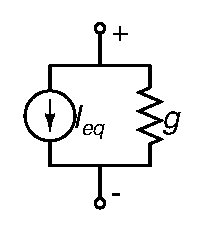
\includegraphics{fig/diode.eps} & 
	\begin{eqnarray*}
		g_{eq}&=&i(v_n)/V_t \\
		I_{eq}&=&i(v_n)-g_{eq}v_n
	\end{eqnarray*}
\end{tabular}
\caption{Linear companion model for diode \label{fig:diode}}
\end{center}
\end{figure}

\pagebreak

\subsection{Metal-Oxide-Silicon Field-Effect Transistor}

The next simplest non-linear devices are n- and p-channel MOSFETs, as no current flows into the gate, and the non-linear source-to-drain port depends on only two parameters, $v_{GS}$ and $v_{DS}$.   The model is complicated slightly, however, by the fact that MOSFETs have three distinct operating regions.  For brevity, we derive only the results for n-channel MOSFETs.  Similar results for p-channel MOSFETs are presented at the end of this subsection.

\subsubsection{Cutoff: $ v_{GS} - V_T < 0 $ }

Cutoff is a trivial operating region, as all of the companion model parameters (depicted in Fig.~\ref{fig:nmos}) zero.  No current flows into any of the nodes.

\begin{figure}[h]
\begin{center}
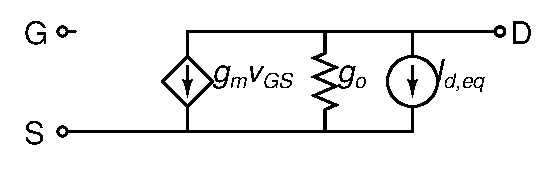
\includegraphics{fig/nmos.eps}
\caption{Linear companion model for n-channel MOSFET \label{fig:nmos}}
\end{center}
\end{figure}

\subsubsection{Saturation: $ 0 \leq v_{GS} - V_T < v_{DS} $}

In saturation, the following large-signal model holds:

\begin{equation}
I_D=\frac{K}{2}(v_{GS}-V_T)^2 (1+(v_{DS}-v_{DS,sat})/V_a)
\end{equation}

where $V_a$ is the Early voltage and  $v_{DS,sat}=v_{GS}-V_T$.  Since $I_D$ is a function of two variables, we now use partial derivatives to find the small-signal conductances across the DS port.

\begin{eqnarray}
g_m&=&\frac{\partial I_D}{\partial v_{GS}}=K(v_{GS}-V_T)(1+(v_{DS}-v_{DS,sat})/V_a)=\sqrt{2KI_D} \\
g_o&=&\frac{\partial I_D}{\partial v_{DS}}=\frac{K}{2}(v_{GS}-V_T)^2 / V_a=I_S/V_a
\end{eqnarray}

We seek to define a bias current from drain to source that will cause the node voltages to evolve by Newton-Raphson iteration, as we did for the diode in the previous subsection.  We now use the multivariable form of the iteration equation:

\begin{equation}
I_{D,n+1}=I_D+g_m(v_{GS,n+1}-v_{GS,n})+g_o(v_{DS,n+1}-v_{DS,n})
\end{equation}

Rearranging this equation, we find that $I_{D,n+1}=(I_D-g_mv_{GS,n}-g_ov_{DS,n})+g_mv_{GS,n+1}+g_ov_{DS,n+1}$.  Hence the bias current is $I_{D,eq}=I_D-g_mv_{GS,n}-g_ov_{DS,n}$.  Although we will not derive it here, it should now be apparent that the following general result holds when dermining bias currents for Newton-Raphson iteration:

\begin{equation}
\label{eqn:bias_current}
I_{eq}=I(\mathcal{V}_i)-\sum_{v \in \mathcal{V}}\frac{\partial I}{\partial v}v_i
\end{equation}

where $\mathcal{V}$ is the set of device port voltages and $\mathcal{V}_i$ is the set of calculated node voltages from the previous iteration.

\subsubsection{Triode: $ 0 \leq v_{DS} \leq v_{GS}-V_T $}

The drain current in this operating region is related to the $v_{GS}$ and $v_{DS}$ by Equation~\ref{eqn:nmos_triode}.  Note that this model does not include the Early effect.

\begin{equation}
\label{eqn:nmos_triode}
I_S=K((v_{GS}-V_T)-v_{DS}/2)v_{DS}
\end{equation}

Applying partial derivatives, we find the small-signal conductances:

\begin{eqnarray}
g_m&=&\frac{\partial I_D}{\partial v_{GS}}=Kv_{DS} \\
g_o&=&\frac{\partial I_D}{\partial v_{DS}}=K((v_{GS}-V_T)-v_{DS})
\end{eqnarray}

Again, $I_{D,eq}=I_D-g_mv_{GS}-g_ov_{DS}$.

\pagebreak

\subsubsection{p-channel Results}

The linear companion model for a p-channel MOSFET is shown in Figure~\ref{fig:pmos}, and the values of $g_m$, $g_o$, and $I_{S,eq}$ for the various operating regions are summarized in Table~\ref{tb:pmos}.  For all operating regions, $I_{S,eq}$ is related to $I_S$, $g_m$, and $g_o$ by the following equation:

\begin{equation}
I_{S,eq} =  I_S - g_m v_{SG} - g_o v_{SD}
\end{equation}

\begin{figure}[h]
\begin{center}
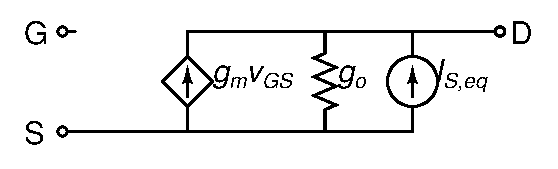
\includegraphics{fig/pmos.eps}
\caption{Linear companion model for p-channel MOSFET \label{fig:pmos}}
\end{center}
\end{figure}

\begin{table}[h]
\caption{PMOS companion model parameters \label{tb:pmos}}
\fbox{
\begin{tabular}[h]{m{4cm}|m{8cm}}
	Operating Region & Parameters \\
	\hline
	\parbox{4cm}{
		Cutoff: \\
		$ v_{SG} - V_T < 0 $ 
	} &
	\begin{eqnarray*}
		I_S &=& 0  \\
		g_m &=& 0  \\
		g_o &=& 0
	\end{eqnarray*} \\
	\hline
	\parbox{4cm}{
		Saturation: \\
		$ 0 \leq v_{GS} - V_T < v_{DS} $
	} &
	\begin{eqnarray*}
		I_S &=& \frac{K}{2} (v_{SG}-V_T)^2(1+(v_{SD}-v_{SD,sat})/V_a) \\
		g_m &=& \sqrt{2KI_S} \\
		g_o &=& I_S/V_a
	\end{eqnarray*} \\
	\hline
	\parbox{4cm}{
		Triode: \\
		$ 0 \leq v_{DS} \leq v_{GS}-V_T $ 
	} &
	\begin{eqnarray*}
		I_S &=& K((v_{SG}-V_T)-v_{SD}/2)v_{SD} \\
		g_m &=& Kv_{SD} \\
		g_o &=& K((v_{SG}-V_T)-v_{SD}) 
	\end{eqnarray*} \\ 
\end{tabular}
}
\end{table}

\pagebreak

\subsection{Bipolar Junction Transistor}

Companion models for BJTs are the most complex circuits presented here because current flows between all nodes.  The model is not quite as unwieldy as it looks, however, because there is only one operating region.

We start with a simplified, mid-band Gummel-Poon NPN model, as shown in Figure~\ref{fig:gummel-poon}.  The base currents are defined as follows:

\begin{eqnarray}
i_{bf}&=&(I_{fs}/\beta_f)(e^{v_{BE}/V_t}-1) \\
i_{br}&=&(I_{rs}/\beta_r)(e^{v_{BC}/V_t}-1)
\end{eqnarray}

Then, defining the small-signal conductances as in Figure~\ref{fig:npn}, we have
\begin{eqnarray}
g_{\pi,f}&=&\frac{\partial i_{bf}}{\partial v_{BE}}=(I_{fs}/\beta_f)e^{v_{BE}/V_t}/V_t \approx I_{bf}/V_t \\
g_{\pi,r}&=&\frac{\partial i_{br}}{\partial v_{BC}}=(I_{rs}/\beta_r)e^{v_{BC}/V_t}/V_t \approx I_{br}/V_t \\
g_{m,f}&=&\frac{\partial i_C}{\partial v_{BE}}=I_{fs}e^{v_{BE}/V_t}/V_t=\beta_fg_{\pi,f} \\
g_{m,r}&=&\frac{\partial i_C}{\partial v_{BC}}=I_{rs}e^{v_{BC}/V_t}/V_t=\beta_rg_{\pi,r}
\end{eqnarray}

We add the Early effect by placing an output resistance across the CE port, with conductance $I_C/V_a$.

Using the general bias current formula (Eqn.~\ref{eqn:bias_current}), we find
\begin{eqnarray}
I_{bf,eq}&=&I_bf(v_{BE})-g_{\pi,f}v_{BE} \\
I_{br,eq}&=&I_br(v_{BC})-g_{\pi,r}v_{BC} \\
I_{C,eq}&=&I_C(v_{BE},v_{BC})-g_{m,f}v_{BE}+g_{m,r}v_{BC}-g_ov_{CE}
\end{eqnarray}

\begin{figure}[h]
\begin{center}
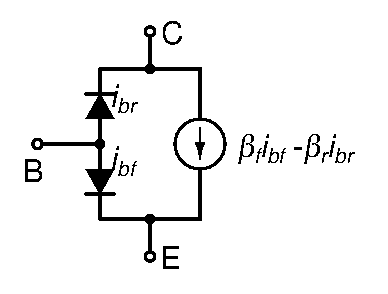
\includegraphics{fig/gummel-poon.eps}
\caption{Mid-band Gummel-Poon BJT Model \label{fig:gummel-poon}}
\end{center}
\end{figure}

\begin{figure}[h]
\begin{center}
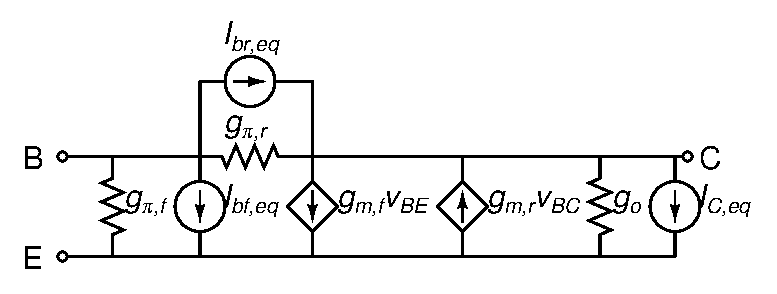
\includegraphics{fig/npn.eps}
\caption{Linear companion model for NPN BJT \label{fig:npn}}
\end{center}
\end{figure}

The analogous model for a PNP BJT is shown in Figure~\ref{fig:pnp}, and the corresponding parameters are listed below:

\begin{eqnarray}
g_{\pi,f}&=&\frac{\partial i_{bf}}{\partial v_{EB}}=(I_{fs}/\beta_f)e^{v_{EB}/V_t}/V_t \approx I_{bf}/V_t \\
g_{\pi,r}&=&\frac{\partial i_{br}}{\partial v_{CB}}=(I_{rs}/\beta_r)e^{v_{CB}/V_t}/V_t \approx I_{br}/V_t \\
g_{m,f}&=&\frac{\partial i_E}{\partial v_{EB}}=I_{fs}e^{v_{EB}/V_t}/V_t=\beta_fg_{\pi,f} \\
g_{m,r}&=&\frac{\partial i_E}{\partial v_{CB}}=I_{rs}e^{v_{CB}/V_t}/V_t=\beta_rg_{\pi,r} \\
g_o&=&I_E/V_a \\
\nonumber \\
I_{bf,eq}&=&I_bf(v_{EB})-g_{\pi,f}v_{EB} \\
I_{br,eq}&=&I_br(v_{CB})-g_{\pi,r}v_{CB} \\
I_{C,eq}&=&I_C(v_{EB},v_{CB})-g_{m,f}v_{EB}+g_{m,r}v_{CB}-g_ov_{EC}
\end{eqnarray}

\begin{figure}[h]
\begin{center}
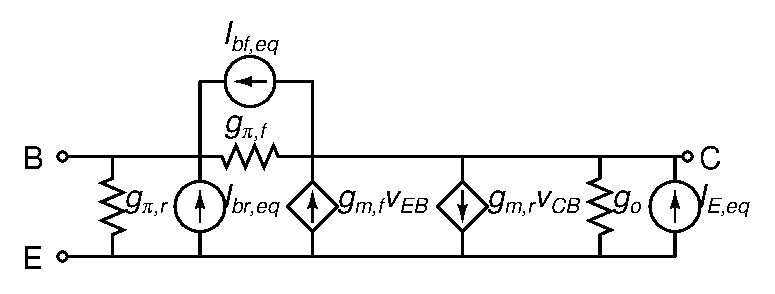
\includegraphics{fig/pnp.eps}
\caption{Linear companion model for PNP BJT \label{fig:pnp}}
\end{center}
\end{figure}

\pagebreak

\section{Energy storage components}
As explained in introduction, transient simulation of energy storage require companion models to be formed. We present here the results for one-step integration methods : Backward Euler (BE), Forward Euler (FE) and Trapezoidal Rule (TR)
\subsection{Capacitor}
In deriving the model parameters, we start with the differential equation relating current to voltage in a capacitor:
\begin{equation}
I=C(dv/dt)
\end{equation}
We then transform this differential equation to an integral equation 
\begin{equation}
v(t+\Delta t) = v(t) + \int_t^{t+\Delta t} i(x) dx
\end{equation}
Then we use an integration method to get an expression for $v_{n+1}$, which can be reformulated as
\begin{equation}
v_{n+1} \approx v_n+(\Delta t/C)I
\end{equation}
How we define $I$ determines the integration method implemented by the companion model. Geometrically, it corresponds to the point at which we evaluate the derivative : FE takes the derivative at the current point, BE at the next point, and TR takes an average of these two. Table~\ref{tb:cap_int} summarizes three common integration methods and the corresponding model parameters.\\
We recognise either a Thevenin model or a voltage source, depending on whether $I$ depends on $I_{n+1}$ (implicit method) or just $I_n$ (explicit method). We should note that every implicit model is represented by a Thevenin model, and can be converted to an equivalent Norton model. We chose Thevenin model for the capacitor since it is more accurate : computers have trouble dividing by small numbers such as $\Delta t$, and this is precisely what Norton models do. This can be explained by the fact that voltage is the state variable of capacitors, so they change proportionally to $\Delta t$.
\begin{table}[h]
\centering
\caption{Capacitor companion model parameters for integration methods \label{tb:cap_int}}
\fbox{
\begin{tabular}{m{4cm}|m{5cm}}

Method & Parameters \\
\hline
\parbox{4cm}{
Forward Euler: \\
$ I=I_{n+1} $
}&
\begin{eqnarray*}
V_{eq}&=&v_{n}+(\Delta t/C)i_{n} \\
R&=&0
\end{eqnarray*} \\

\hline
\parbox{4cm}{
Backward Euler: \\
$ I=I_n $
}&
\begin{eqnarray*}
V_{eq}&=&v_{n} \\
R&=&\Delta t/C
\end{eqnarray*} \\

\hline
\parbox{4cm}{
Trapezoidal: \\
$ I=(I_n+I_{n+1})/2 $
}&
\begin{eqnarray*}
V_{eq}&=&v_{n}+(\Delta t/2C)i_{n} \\
R&=&\Delta t/2C
\end{eqnarray*}

\end{tabular}}
\end{table}

\begin{figure}[h]
\begin{center}
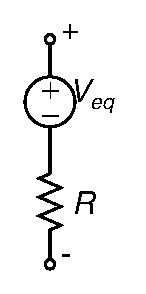
\includegraphics{fig/cap.eps}
\caption{Linear companion model for capacitor \label{fig:cap}}
\end{center}
\end{figure}

\pagebreak

\subsection{Inductor}
The inductor is the dual of the capacitor, so similar results apply. We end up with the formula
\begin{equation}
i_{n+1} \approx i_n + (\Delta t/L)V
\end{equation}
Where $V$ is determined by the integration method. The results are displayed in Table~\ref{tb:inductor_int}. Again, we have the choice between Thevenin and Norton model for implicit methods, and for the same reasons, we choose Norton model (current is the state variable of the inductor).

\begin{table}[h]
\caption{Induction companion model parameters for integration methods \label{tb:inductor_int}}
\centering
\fbox{
\begin{tabular}{m{4cm}|m{5cm}}

Method & Parameters \\
\hline
\parbox{4cm}{
Forward Euler: \\
$ V=V_{n+1} $
}&
\begin{eqnarray*}
I_{eq}&=&i_{n}+(\Delta t/L)v_{n} \\
g&=&0
\end{eqnarray*} \\

\hline
\parbox{4cm}{
Backward Euler: \\
$ V=V_n $
}&
\begin{eqnarray*}
I_{eq}&=&i_{n} \\
R&=&\Delta t/L
\end{eqnarray*} \\

\hline
\parbox{4cm}{
Trapezoidal: \\
$ V=(V_n+V_{n+1})/2 $
}&
\begin{eqnarray*}
I_{eq}&=&i_{n}+(\Delta t/2L)v_{n} \\
R&=&\Delta t/2L
\end{eqnarray*}
\end{tabular}}
\end{table}

\begin{figure}[h]
\begin{center}
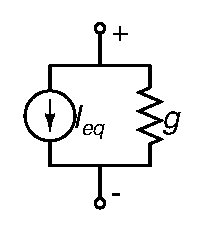
\includegraphics{fig/inductor.eps}
\caption{Linear companion model for inductor \label{fig:inductor}}
\end{center}
\end{figure}

\pagebreak

\nocite{*}
\bibliography{lec}

\end{document}
